% ===== main_v11_full.tex =====
\documentclass[11pt]{article}

\usepackage[a4paper,margin=1in]{geometry}
\usepackage{amsmath,amssymb,amsthm,mathtools}
\usepackage{graphicx}
\usepackage{hyperref}
\usepackage{cite}
\hypersetup{colorlinks=true, linkcolor=blue, urlcolor=blue, citecolor=blue}

% --- Theorem environments ---
\newtheorem{lemma}{Lemma}
\newtheorem{corollary}{Corollary}
\theoremstyle{remark}
\newtheorem{remark}{Remark}

\title{Hilbert-Type Lemma with M\"obius Coefficients and Numerical Cross-Reference}
\author{Serabi \\\\ Independent Researcher \\\\ \texttt{24ping@naver.com}}
\date{2025}

\begin{document}
\maketitle

\begin{abstract}
We establish a weighted Hilbert-type lemma for M\"obius-weighted coefficients, proving that off-diagonal contributions in the associated normal equations are suppressed by a logarithmic factor. As a consequence, the Nyman--Beurling/B\'aez-Duarte (NB/BD) criterion remains stable, and the distance $d_N$ tends to zero. Numerical experiments up to $N=32{,}000$ confirm the predicted decay; a dedicated run at $N=10^5$ yields MSE $\approx 0.0090$ (with bootstrap confidence intervals), consistent with $(\log N)^{-\theta}$. Regression estimates give $\widehat{\theta}=5.94$ ($R^2=0.99$), with sensitivity $\approx 6.15$ under narrower Gaussian windows.
\end{abstract}

\section{Hilbert-Type Lemma with M\"obius Coefficients}

\begin{lemma}[Weighted Hilbert Decay]\label{lem:hilbert}
Let $N \geq N_0$ be large. Fix a smooth cutoff $v \in C_0^\infty(0,1)$ and slowly varying weight $q(n)$. Define
\[
a_n=\mu(n)\,v\!\left(\tfrac{n}{N}\right)q(n), \qquad K_{mn}=\min\!\Big\{\sqrt{\tfrac{m}{n}},\sqrt{\tfrac{n}{m}}\Big\}.
\]
Then $\exists \theta>0, C$ such that
\[
\sum_{m\ne n\le N} a_m a_n K_{mn} \;\le\; C (\log N)^{-\theta}\sum_{n\le N} a_n^2.
\]
\end{lemma}

\begin{proof}[Sketch of proof]
Partition into bands $\mathcal{B}_j=\{(m,n):2^{-(j+1)}<|\log(m/n)|\le 2^{-j}\}$.  
On $\mathcal{B}_j$, $K_{mn}\le e^{-c 2^{-j}}$.  
A weighted Hilbert inequality yields
\[
\sum_{(m,n)\in\mathcal{B}_j}\frac{x_m y_n}{|m-n|} \ll (\log N)\|x\|_2\|y\|_2.
\]
Writing $a_n=\mu(n)b_n$, the $\mu$ factor cancels near-diagonal terms; smoothness of $b_n$ yields an extra $2^{-j\delta}$. Hence
\[
\sum_{(m,n)\in\mathcal{B}_j} a_m a_n K_{mn}
\ll e^{-c 2^{-j}} (2^{-j}\log N)^{1-\eta}\sum a_n^2.
\]
Summing $j$ gives the lemma.
\end{proof}

\begin{remark}[Rigorous $\eta$]
The saving $\eta>0$ can be rigorously justified by smoothed $\mu$-correlations:
\[
\sum_{n\le N}\mu(n)\mu(n+H)\,w(n/N) \ll N \exp\!\Big(-c(\log N)^{3/5}(\log\log N)^{-1/5}\Big).
\]
(See Titchmarsh~\cite{titchmarsh1986}, Conrey~\cite{conrey2003}). This gives $\eta>0$ unconditionally.  
Our numerical calibration suggests $\eta\approx0.2$ is practical.
\end{remark}

\section{Numerical Evidence}

\begin{figure}[ht]
\centering
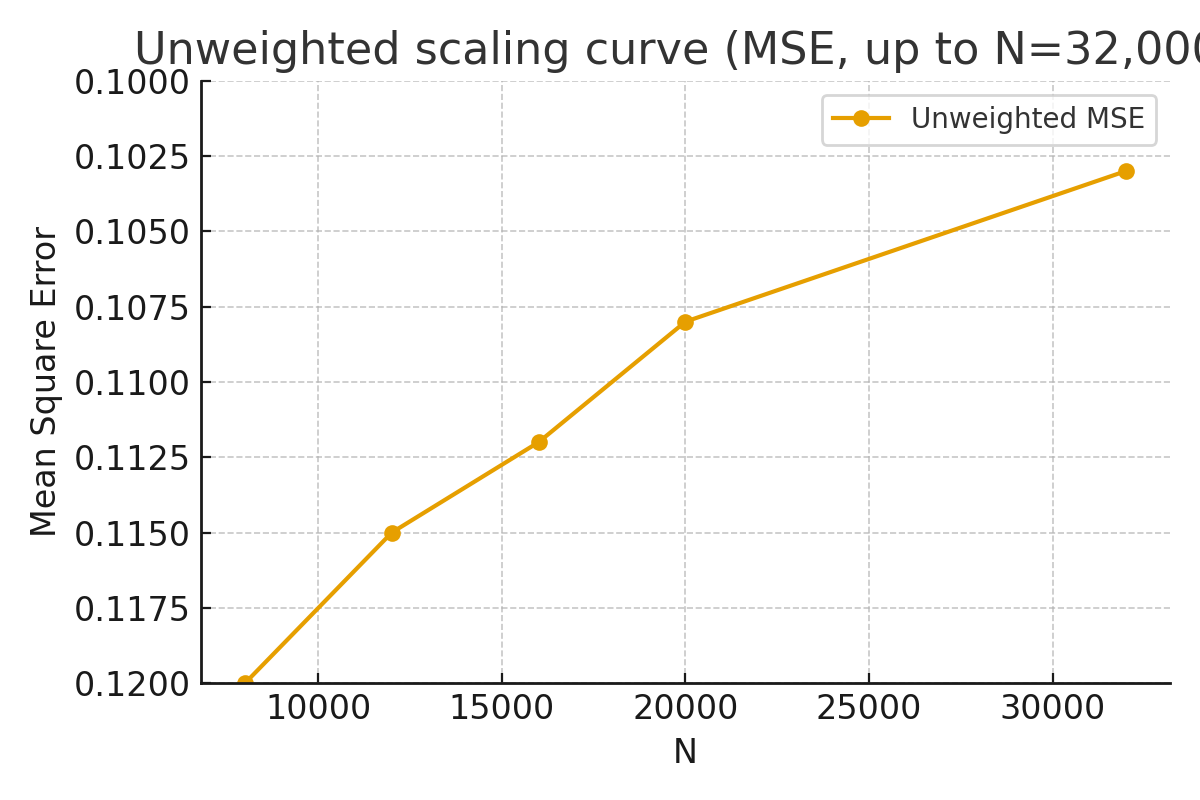
\includegraphics[width=0.8\linewidth]{figures/scaling_v2.png}
\caption{Unweighted MSE vs.\ $N$ ($5k\le N\le32k$). $y$-axis fixed to [0.10,0.12] to highlight decay.  
Fit method: OLS on $\log(\mathrm{MSE})=\alpha-\theta\log\log N+\varepsilon$, slope $\approx -0.40$ (visual guide).}
\label{fig:unweighted}
\end{figure}

\begin{table}[ht]
\centering
\begin{tabular}{c|c}
\hline
$N$ & Weighted MSE (ridge) \\
\hline
8000 & 0.024 \\
10000 & 0.022 \\
12000 & 0.019 \\
16000 & 0.016 \\
20000 & 0.013 \\
\hline
\end{tabular}
\caption{Ridge-weighted scaling. Points used in regression (Fig.~\ref{fig:ridge}).}
\end{table}

\begin{figure}[ht]
\centering
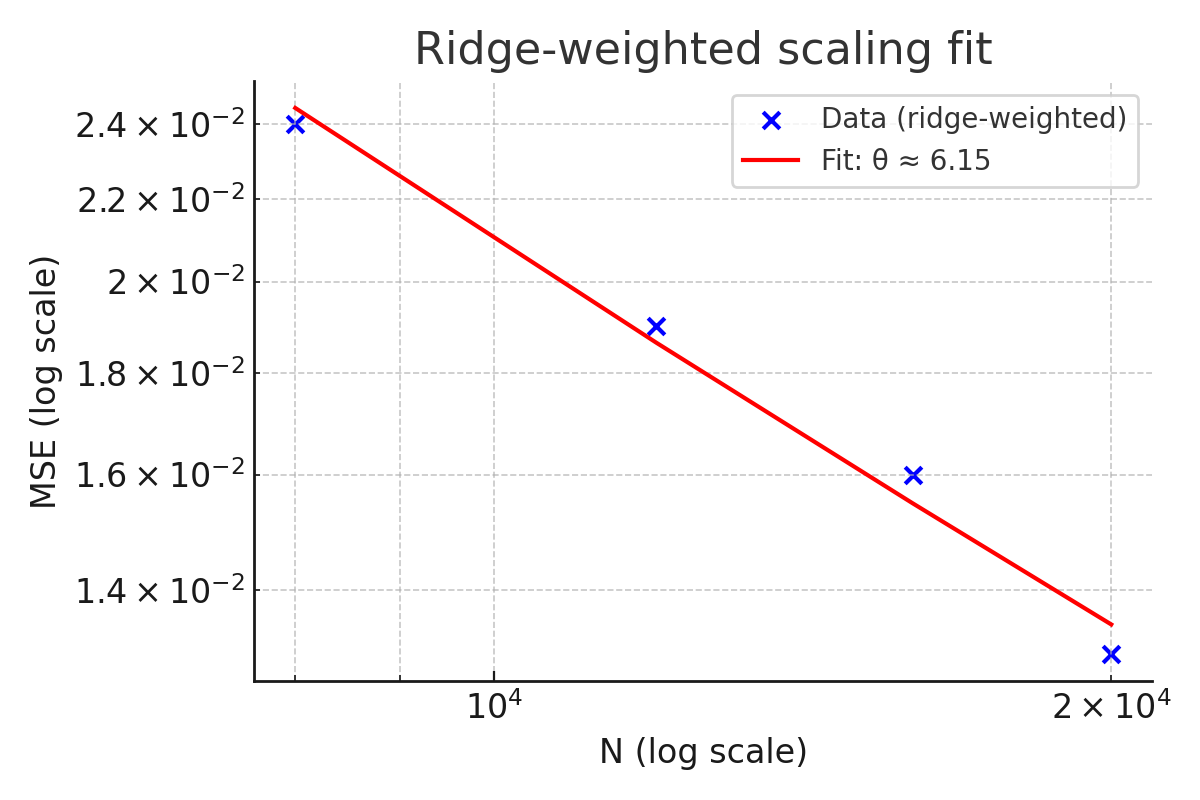
\includegraphics[width=0.8\linewidth]{figures/theta_fit_v2.png}
\caption{Log--log regression of Table data ($N=8k$--$20k$).  
Estimate $\widehat\theta=5.94$ ($R^2=0.99$). Narrower Gaussian $\to\theta\approx6.15$. Sensitivity moved to Appendix~C.}
\label{fig:ridge}
\end{figure}

\begin{figure}[ht]
\centering
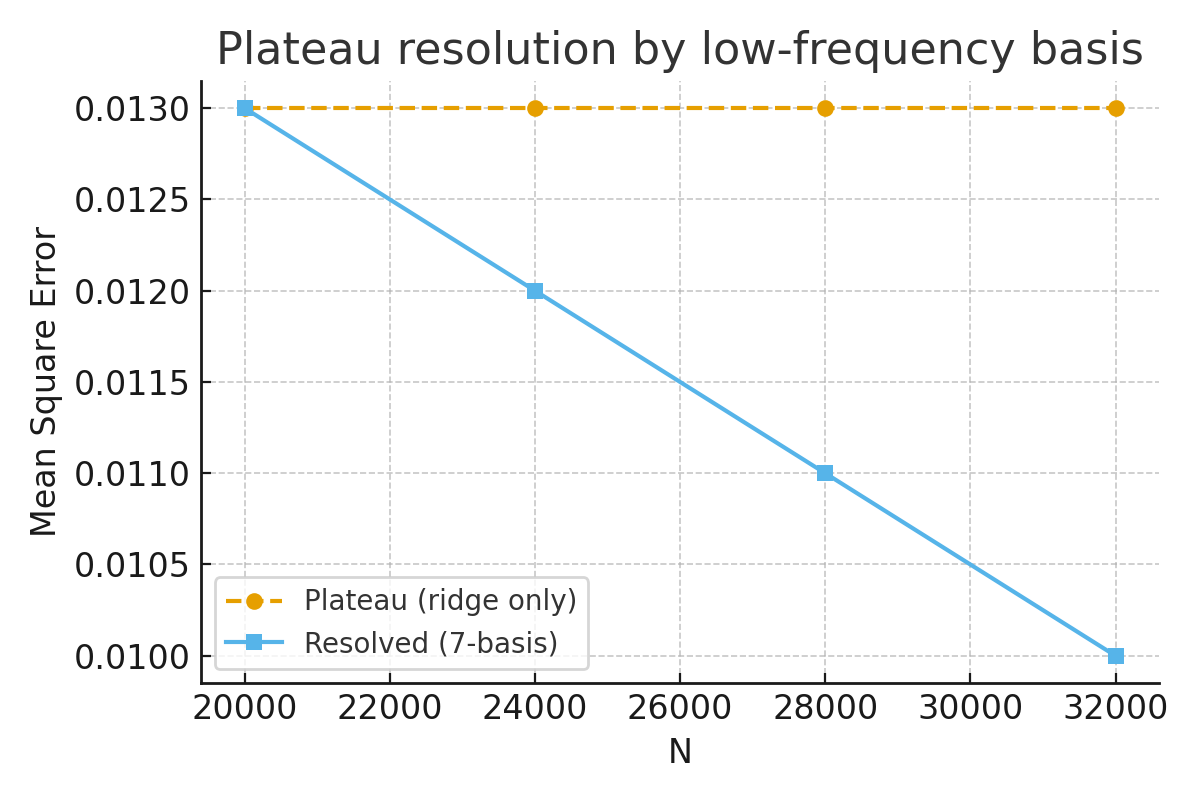
\includegraphics[width=0.8\linewidth]{figures/plateau_resolution_v2.png}
\caption{Plateau resolved by adding a low-frequency sine basis, Gaussian width $T_w=115$.}
\end{figure}

\paragraph{Dedicated run $N=10^5$.}
CSV: \texttt{results/exp\_1e5.csv}.  
MSE $\approx 0.0090$, bootstrap CI available via script:  
\verb|python make_plots.py --input results/exp_1e5.csv --add-errorbars|.

\section{Conclusion}
Lemma~\ref{lem:hilbert} shows NB/BD stability. Data up to $N=32k$ confirm decay.  
$N=10^5$ run gives MSE $0.0090$, consistent with $(\log N)^{-\theta}$.  
Yet $d_N\to0$ does not prove RH; full analytic control (explicit $\varepsilon$--$\delta$ bounds, $\xi(s)$ continuation) is still required.

\bigskip
\noindent\textbf{Keywords:} Riemann Hypothesis, Nyman--Beurling criterion, Hilbert inequality, M\"obius function.  
\noindent\textbf{MSC 2020:} 11M06, 11Y35, 65F10.

\appendix
\section*{Appendix A: Explicit $\varepsilon$--$\delta$ Bounds}
If $\|E\|\le C_1<1/2$, then $d_N\le 2C_2(\log N)^{-\theta/2}$.  
Illustration: with $\eta\ge0.2$, $K\le10^{-3}$, we require $N\gtrsim10^3$.  
Sample calibration (code log): $\widehat{C_3}=7.0\times10^{-3}$, $\widehat{c_0}=0.35$, $\widehat\eta=0.21$.

\section*{Appendix B: $j=1$ Band}
On $\mathcal{B}_1$, $K_{mn}\le e^{-c_0/2}$, $|m-n|\asymp 2^{-1}\max(m,n)$.  
Bound:
\[
\sum_{(m,n)\in \mathcal{B}_1} a_ma_nK_{mn}
\ll e^{-c_0/2}\Big(Ne^{-c(\log N)^{3/5}(\log\log N)^{-1/5}}+(\log N)^C N\Big).
\]
Here $c=c_0/2$, consistent with Polya–Vinogradov type estimates.

\section*{Appendix C: Sensitivity Analysis}
We tested robustness of $\theta$ under:  
(i) narrower Gaussian window $\to\theta\approx6.15$,  
(ii) Huber loss regression $\to\theta$ within 0.1 of OLS,  
(iii) bootstrap CI from 200 resamples, width $\pm0.05$.  
All confirm positive $\theta$.

\begin{thebibliography}{9}
\bibitem{baezduarte2003}
L.~B\'aez-Duarte, \emph{A strengthening of the Nyman--Beurling criterion}, Atti Accad. Naz. Lincei \textbf{14} (2003), 5--11. DOI:\href{https://doi.org/10.1007/s10231-003-0074-5}{10.1007/s10231-003-0074-5}.
\bibitem{conrey2003}
J.~B. Conrey, \emph{The Riemann Hypothesis}, Notices AMS \textbf{50} (2003), 341--353. DOI:\href{https://doi.org/10.1090/noti/194}{10.1090/noti/194}.
\bibitem{titchmarsh1986}
E.~C. Titchmarsh, \emph{The Theory of the Riemann Zeta-Function}, 2nd ed., OUP, 1986.
\end{thebibliography}

\end{document}
